\documentclass[a4paper]{report}
\usepackage{hyperref}
\usepackage{parskip}
\usepackage{graphicx}
\usepackage{a4wide}
\usepackage{wrapfig}
\usepackage{subfig}
\usepackage{groove2tikz}
\usepackage[all]{xy}
\usepackage{mathtools}
\usepackage{amssymb}
\usepackage{multirow}
\usepackage{array}
\usepackage{amsthm}
\usepackage{fancybox}
\usepackage{verbatim}

% Macro for 'List of Symbols', 'List of Notations' etc...
%LTS
\newcommand{\States}{Q}
\newcommand{\state}{q}
\newcommand{\Labels}{L}
\newcommand{\ltsLabel}{l}
\newcommand{\Transitions}{T}
\newcommand{\transition}{t}
\newcommand{\initialState}{q_0}

%Algebra
\newcommand{\Sorts}{S}
\newcommand{\sort}{s}
\newcommand{\sortFunction}{\sigma}

\newcommand{\FunctionSymbols}{F}
\newcommand{\functionSymbol}{f}

\newcommand{\Algebra}{\mathcal{A}}

\newcommand{\Functions}{\Phi}
\newcommand{\function}{\phi}

\newcommand{\Variables}{\mathcal{V}}
\newcommand{\DefinedVariables}{V}
\newcommand{\variable}{v}

\newcommand{\Terms}{\mathcal{T}}
\newcommand{\term}{t}
\newcommand{\BooleanTerms}{\mathcal{B}}
\newcommand{\termMapping}{\mu}
\newcommand{\valuation}{\nu}

%STS
\newcommand{\Locations}{W}
\newcommand{\location}{w}
\newcommand{\initialLocation}{\location_0}
\newcommand{\LocationVariables}{\mathcal{L}}
\newcommand{\InteractionVariables}{\mathcal{I}}
\newcommand{\initializationFunction}{\imath}
\newcommand{\Gates}{\Lambda}
\newcommand{\gate}{\lambda}
\newcommand{\Switches}{D}
\newcommand{\switch}{d}
\newcommand{\guard}{\gamma}
\newcommand{\updateMapping}{\rho}

\newcommand{\StsExpansionMapping}{\mu}

% Graph Grammars
\newcommand{\Nodes}{\mathbb{V}}
\newcommand{\Edges}{\mathbb{E}}
\newcommand{\GraphNodes}{\mathbb{W}}
\newcommand{\hostGraph}{G}
\newcommand{\DefinedNodes}{V}
\newcommand{\DefinedEdges}{E}
\newcommand{\DefinedHostNodes}{\DefinedNodes_{\hostGraph}}
\newcommand{\DefinedHostEdges}{\DefinedEdges_{\hostGraph}}
\newcommand{\ruleGraph}{H}
\newcommand{\DefinedRuleNodes}{\DefinedNodes_{\ruleGraph}}
\newcommand{\DefinedRuleEdges}{\DefinedEdges_{\ruleGraph}}
\newcommand{\edge}{e}
\newcommand{\node}{z}
\newcommand{\TermNodes}{2^\Terms}
\newcommand{\RulePriorities}{P}
\newcommand{\rulePriority}{p}


% GTS
\newcommand{\Graphs}{\mathcal{G}}
\newcommand{\Rules}{R}
\newcommand{\ggrule}{r}
\newcommand{\RuleMatches}{M}
\newcommand{\rulematch}{m}
\newcommand{\RuleTransitions}{U}
\newcommand{\ruleTransition}{u}
\newcommand{\startGraph}{G_0}

% point algebra
\newcommand{\PointAlgebra}{\mathcal{P}}

%IO
\newcommand{\IOTypes}{Y}
\newcommand{\iotype}{\iota}
\newcommand{\IOTransitions}{\Transitions_{\IOTypes}}
\newcommand{\IOGates}{\Gates_{\IOTypes}}
\newcommand{\IORules}{\Rules_{\IOTypes}}
\newcommand{\IOLabels}{\Labels_{\IOTypes}}
\newcommand{\IORuleTransitions}{\RuleTransitions_{\IOTypes}}

% GG variable
\newcommand{\variableAnchor}{\node_a}
\newcommand{\valueEdge}{\edge_v}
\newcommand{\variableLabel}{\ltsLabel_a}
\newcommand{\valueLabel}{\ltsLabel_v}
\newcommand{\GGVariables}{\Variables_{GG}}

\def\listofsymbols{\begin{tabbing}
% LTS
% YOU NEED TO ADD THE FIRST ONE MANUALLY TO ADJUST THE TABBING AND SPACES
$\States$~~~~~\=\parbox{5in}{Set of states\dotfill \pageref{symbol:States}}\\
\addsymbol \Labels: {Set of labels}{symbol:Labels}
\addsymbol \Transitions: {Set of transitions}{symbol:Transitions}
\addsymbol \initialState: {Initial state}{symbol:initialState}

% IO
\addsymbol \IOTypes: {Input/Output type}{symbol:IOTypes}

% Algebra
\addsymbol \Sorts: {Set of sorts}{symbol:Sorts}
\addsymbol \FunctionSymbols: {Set of function symbols}{symbol:FunctionSymbols}
\addsymbol \Functions: {Set of functions}{symbol:Functions}

\addsymbol \Variables: {Set of variables}{symbol:Variables}
\addsymbol \Terms: {Set of terms}{symbol:Terms}
\addsymbol \termMapping: {Term-mapping function}{symbol:termMapping}
\addsymbol \valuation: {Valuation function}{symbol:valuation}

% STS
\addsymbol \Locations: {Set of locations}{symbol:Locations}
\addsymbol \initialLocation: {Initial location}{symbol:initialLocation}
\addsymbol \LocationVariables: {Set of location variables}{symbol:LocationVariables}
\addsymbol \InteractionVariables: {Set of interaction variables}{symbol:InteractionVariables}
\addsymbol \initializationFunction: {Term mapping for location variable initialization}{symbol:initializationFunction}
\addsymbol \Gates: {Set of gates}{symbol:Gates}
\addsymbol \Switches: {Set of switch relations}{symbol:Switches}
\addsymbol \guard: {Guard of a switch relation}{symbol:guard}
\addsymbol \updateMapping: {Update mapping of a switch relation}{symbol:updateMapping}

% Graph grammar

\end{tabbing}
 \clearpage}
\def\addsymbol #1: #2#3{$#1$ \> \parbox{5in}{#2 \dotfill \pageref{#3}}\\} 
\def\newnot#1{\label{#1}} 

\graphicspath{{./img/}}
%\renewcommand*\familydefault{\sfdefault}

\hypersetup{pdfborder = {0 0 0 0}}

\setcounter{tocdepth}{3}
\setcounter{secnumdepth}{4}

\theoremstyle{definition}
\newtheorem{definition}{Definition}[section]

\begin{document}
	\title{\textbf{Model-Based Testing with\\Graph Grammars}}
	\author{\textbf{MSc Thesis} \textit{(Afstudeerscriptie)}\\
	\\
	written by
	\\
	\\
	Vincent de Bruijn\\
	\\
	Formal Methods \& Tools,\\
	University of Twente,
	\\Enschede,\\
	The Netherlands\\
	\\
	\texttt{v.debruijn@student.utwente.nl}}
	\date{\today}
	\maketitle
	
	\begin{abstract}
\textit{Graph Grammars} have many structural advantages, which are potential benefits for the model-based testing process. We describe a model-based testing setup with Graph Grammars. The result is a system for automatic test generation from Graph Grammars. A graph transformation tool, GROOVE, and a model-based testing tool, ATM, are used as the backbone of the system. The system is validated using the results of several case studies.
\end{abstract}

	
	\newpage
	\tableofcontents
  \newpage

  \newpage
	\chapter{Introduction}\label{chapter:introduction}
	
	In this introduction, first the importance of testing and automation of testing is stressed. Then Model-Based Testing is shown to be a useful tool for automation of testing. Graph Grammars and graph transformation are argued to be useful as formalism for Model-Based Testing. Some leading tools for automatic test generation are set out, which include the tools used in this report. The research goals are given and finally a roadmap explains the basic structure of the rest of this report.

\section{Testing}
In software development projects, often time and budget costs are exceeded. Laird and Brennan~\cite{Laird:SoftwareMeasurement} investigated in 2006 that 23\% of all software projects are canceled before completion. Furthermore, of the completed projects, only 28\% are delivered on time with the average project overrunning the budget with 45\%. The cause of this often are the unclear ambigious requirements of the software system to develop.

Testing is an important part of software development, because it decreases future maintainance costs~\cite{McConnell:testing}. Testing is a complex process and should be done often~\cite{Pol:testing}. Therefore, the testing process should be as efficient as possible in order to save resources.

Test automation allows repeated testing during the development process. The advantage of this is that bugs are found early and can therefore be fixed early.  A widely used practice is maintaining a \textit{test suite}, which is a collection of test-cases. However, when the creation of a test suite is done manually, this still leaves room for human error~\cite{Blackburn:testing}. The process of deriving tests tends to be unstructured, barely motivated in the details, not reproducible, not documented, and bound to the ingenuity of single engineers~\cite{Utting:MBTTaxonomy}.

\section{Model-based Testing}
The existence of an artifact that explicitly encodes the intended behaviour can help mitigate the implications of these problems. Creating an abstract representation or a \textit{model} of the system is an example of such an artifact. What is meant by a model in this report, is the description of the behavior of a system. In particular, the term model will be often used to describe transition-based notations, such as finite state machines, labelled transition systems and I/O automata. Other notations, such as UML statecharts, are not considered as models in this report. 

A model can be used to systematically generate tests for the system. This is referred to as \textit{model-based testing}. Generating tests automatically leads to a larger test suite than if done manually. A large, systematically built test suite is bound to find more bugs than a smaller, manually built one.

Models are created from the specification documents provided by the end-user. These specification documents are 'notoriously error-prone'~\cite{McCabe:testing}. This implies that the model itself needs validation. Validating the model usually means that the requirements themselves are scrutinised for consistency and completeness~\cite{Utting:MBTTaxonomy}. This helps to clear up ambigious requirements early on, which allows better estimation of the budget and time demands.

The stakeholders evaluate the constructed model to verify its correctness. However, the visual or textual representation of large models may become troublesome to understand, which is referred to as the model having a low model transparency or high model complexity. The problem with transition systems is that a larger number of states and/or transitions decreases the model transparency. We think that low model transparency make errors harder to detect and that it obstructs the feedback process of the stakeholders. Using models with high transparency is therefore essential.

\section{Graph Transformation}
A formalism that claims to have more model transparency is Graph Transformation. The system states are represented by graphs and the transitions between the states are accomplished by applying graph change rules to those graphs. These rules can be expressed as graphs themselves. A graph transformation model of a software system is therefore a collection of graphs, each a visual representation of one aspect of the system. This formalism may therefore provide a more intuitive approach to system modelling than traditional state machines. Graph Transformation and its potential benefits have been studied since the early '70s. The usage of this computational paradigm is best described by the following quote from Andries et al.~\cite{Andries1999}: \begin{quote}Graphs are well-known, well-understood, and frequently used means to represent system states, complex objects, diagrams, and networks, like flowcharts, entity-relationship diagrams, Petri nets, and many more. Rules have proved to be extremely useful for describing computations by local transformations: Arithmetic, syntactic, and deduction rules are well-known examples.\end{quote} An informative paper on graph transformations is written by Heckel et al.~\cite{Heckel2006187}. A quote from this paper: \begin{quote}Graphs and diagrams provide a simple and powerful approach to a variety of problems that are typical to computer science in general, and software engineering in particular.\end{quote}

\section{Tools}
Tools for automatic test generation already exist. The testing tool developed by Axini\footnote{http://www.axini.nl/} is used for the automatic test generation on \textit{symbolic} models, which combine a state and data type oriented approach. This tool is used in this report and is referred to as Axini Test Manager (ATM). In Utting et al.~\cite{Utting:MBTTaxonomy}, a taxonomy is done on different model-based testing tools:
\begin{itemize}
  \item TorX~\cite{Tretmans:TorX}: accepts behaviour models such as I/O labelled transition systems. A version of this tool written in Java under continuous development is JTorX~\cite{Belinfante:JTorX}. This version accepts the same kind of models as ATM.
  \item Spec Explorer\cite{Veanes:SpecExplorer}: provides a model editing, composition, exploration and visualization environment within Visual Studio, and can generate offline .NET test suites or execute tests as they are generated (online).
  \item JUMBL\cite{Prowell:JUMBL}: an academic model-based statistical testing that supports the development of statistical usage-based models using Markov chains, the analysis of models, and the generation of test cases.
  \item AETG\cite{Cohen:AETG}: implements combinatorial testing, where the number of possible combinations of input variables are reduced to a few 'representative' ones.
  \item STG tool\cite{clarke:STG}: implements conformance testing techniques to automatically derive symbolic test cases from formal operational specifications.
\end{itemize}

The graph transformation tool GROOVE\footnote{http://sourceforge.net/projects/groove/} is used to model and explore graph grammars.\marginpar{Zijn er nog andere graph transformation tools?}

\section{Research goals}\label{sec:goals}
The motivation above is given for using graph grammars as a modelling technique. The goal of this research is to create a system for automatic test generation on graph grammars. If the assumptions that graph grammars provide a more intuitive modelling and testing process hold, this new testing approach will lead to a more efficient testing process and fewer incorrect models. The system to be designed, once implemented and validated, should provide a valuable contribution to the testing paradigm. The tools GROOVE and ATM are used to create this system.

The research goals are split into a design and validation component:
\begin{enumerate}
    \item \textbf{Design}: Design and implement a system using ATM and GROOVE which performs model-based testing on graph grammars.
    \item \textbf{Validation}: Validate the design and implementation using case studies and performance measurements.
\end{enumerate}

The result of the design goal is one system called the GROOVE-Axini Testing System (GRATiS). The validation goal uses case-studies with existing specifications from systems tested by Axini. Each case-study has a graph grammar and a symbolic model which describe the same system. GRATiS and ATM are used for the automatic test generation on these models respectively. Both the models and the test processes are compared as part of the validation.

The solution has to uphold three requirements:
\begin{enumerate}
\item A graph grammar must be used as the model; it must derive from the specification and be used for the testing.
\item It must be possible to measure the test progress/completion, by means of \textit{coverage} statistics (explained in detail in section~\ref{sec:coverage}).
\item The solution must be efficient: it should be usable in practice, therefore the technique should be scalable and the imposed constraints reasonable from a practical view point.
\end{enumerate}

\section{Roadmap}
This report has five more chapters: first, the concepts described in this chapter are elaborated in chapter \ref{chapter:background}. The design of GRATiS is described in chapter \ref{chapter:gg_to_sts}. The implementation of GRATiS is covered in chapter~\ref{chapter:implementation}. The validation of GRATiS is in chapter \ref{chapter:validation}. Finally, conclusions are drawn in chapter \ref{chapter:conclusion}. \marginpar{hoofdstukken met ?? zitten niet in dit verslag}

	%\section{Research Goals}\label{sec:goals}

The research goals are split into a design and validation component:
\begin{enumerate}
    \item \textbf{Design}: Design and implement a system using ATM and GROOVE which performs model-based testing on graph grammars.
    \item \textbf{Validation}: Validate the design and implementation using case studies and performance measurements.
\end{enumerate}

The result of the design goal is one system called the GROOVE-Axini Testing System (GRATiS). The validation goal uses case-studies with existing specifications from systems tested by Axini. Each case-study has a graph grammar and a symbolic model which describe the same system. GRATiS and ATM are used for the automatic test generation on these models respectively. Both the models and the test processes are compared as part of the validation.

	
	\newpage
	\chapter{Background}\label{chapter:background}
	The structure of the rest of this chapter is as follows: the general model-based testing process is set out in section \ref{sec:model_based_testing}. Some basic concepts from algebra are described in section~\ref{sec:algebra}. The symbolic models from ATM are then described in section \ref{sec:symbolic}. Section \ref{sec:graph} describes the graph grammar formalism. GROOVE and ATM are described in section \ref{sec:tooling}.

	
	\section{Model-based Testing}\label{sec:model_based_testing}

Model-based testing is a testing technique where a System Under Test (SUT) is tested for conformance to a model description of the system. The general setup for this process is depicted in Figure~\ref{fig:model_based_testing}. The specification of a system, given as a model, is given to a test derivation component which generates test cases. These test cases are passed to a component that executes the test cases on the SUT. Tests are executed by providing input/stimuli to the SUT and monitoring the output/response. The test execution component evaluates the test cases, the stimuli and the responses. It gives a 'pass' or 'fail' verdict depending on whether the SUT conforms to the specification or not respectively.

\begin{figure}[ht]
  \begin{center}
    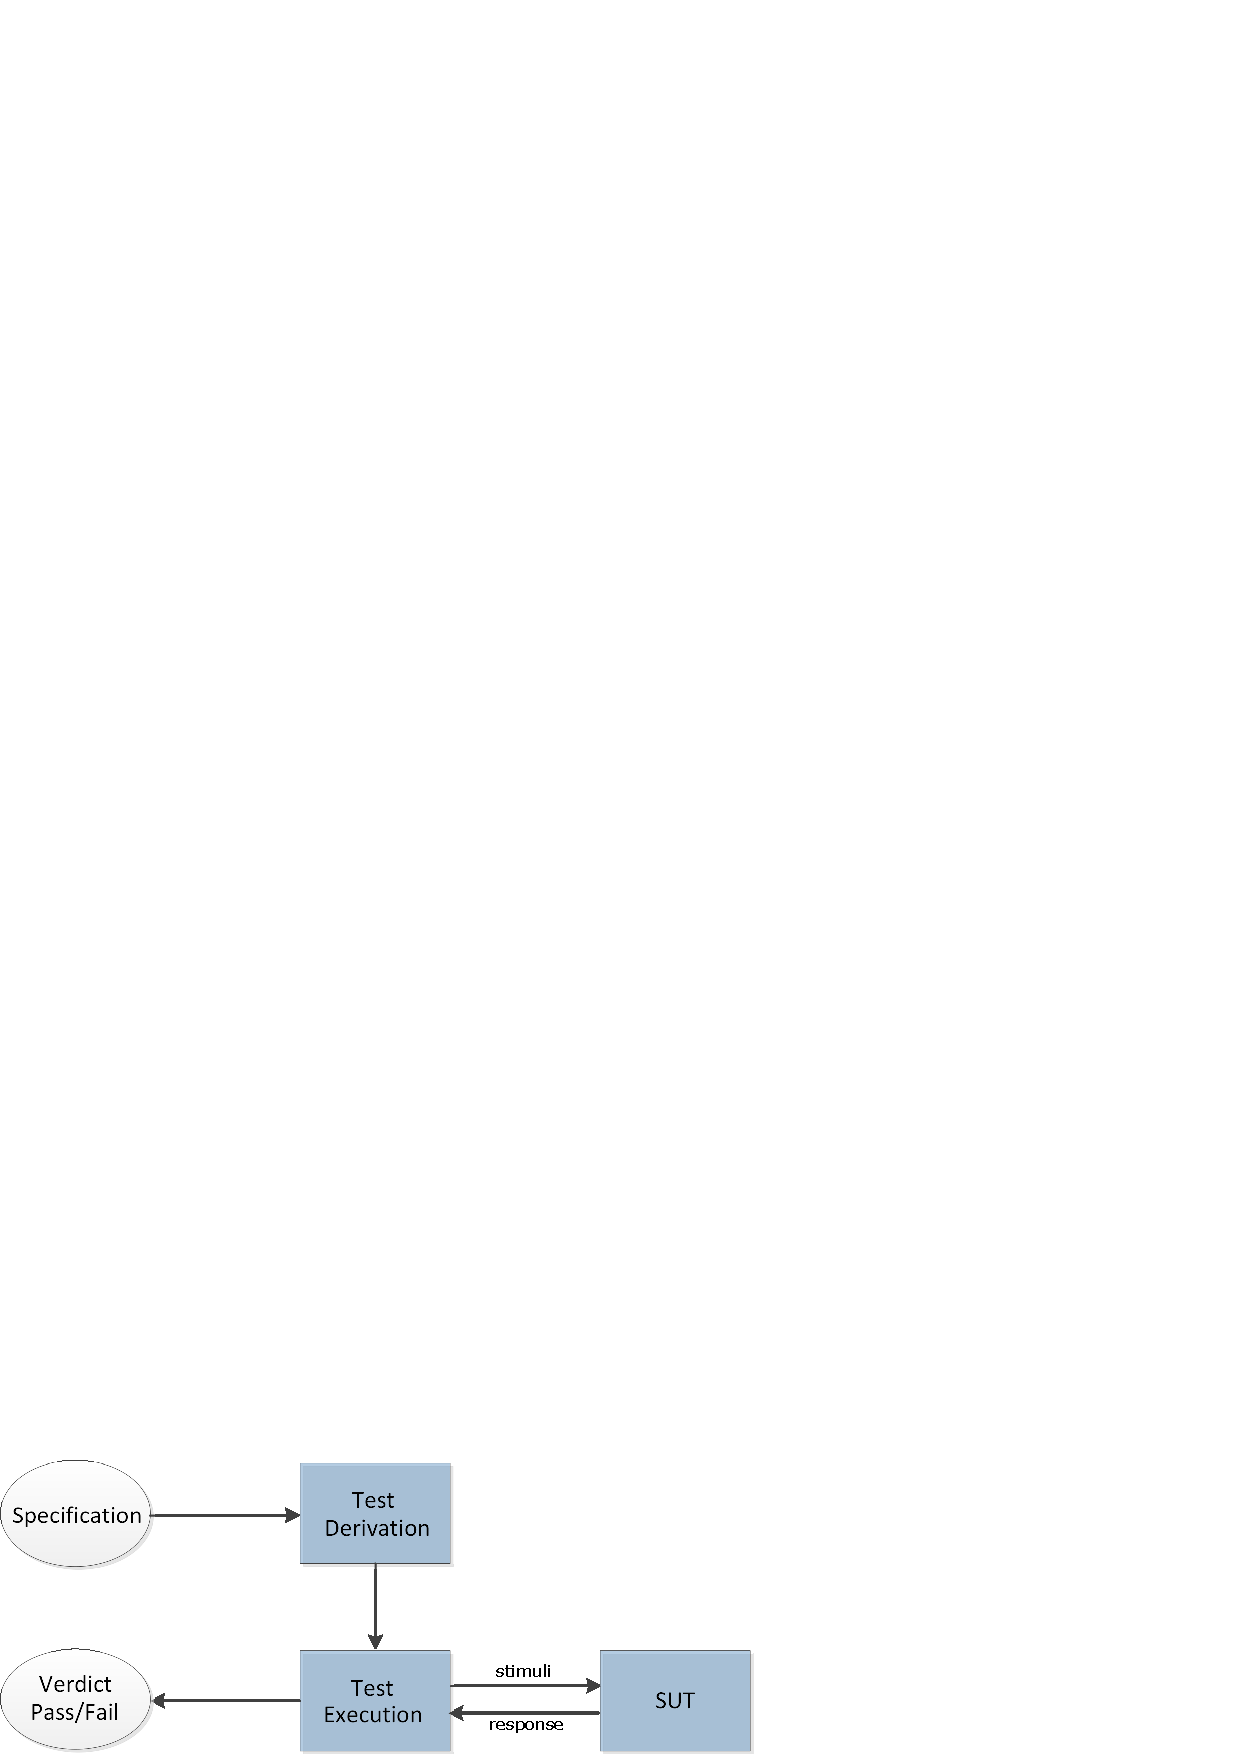
\includegraphics[width=0.75\textwidth]{model-based-testing.pdf}
  \end{center}
  \caption{A general model-based testing setup}
  \label{fig:model_based_testing}
\end{figure}

This type of model-based testing is called \textit{batch testing} or \textit{offline testing}. Another type of model-based testing is \textit{on-the-fly} testing. The main difference is that no test cases are derived, instead a transition in the model is chosen and tested on the system directly. The general architecture for this process is shown in Figure~\ref{fig:model_based_testing_on_the_fly}. An example of an on-the-fly testing is TorX~\cite{Tretmans:TorX}.

\begin{figure}[ht]
  \begin{center}
    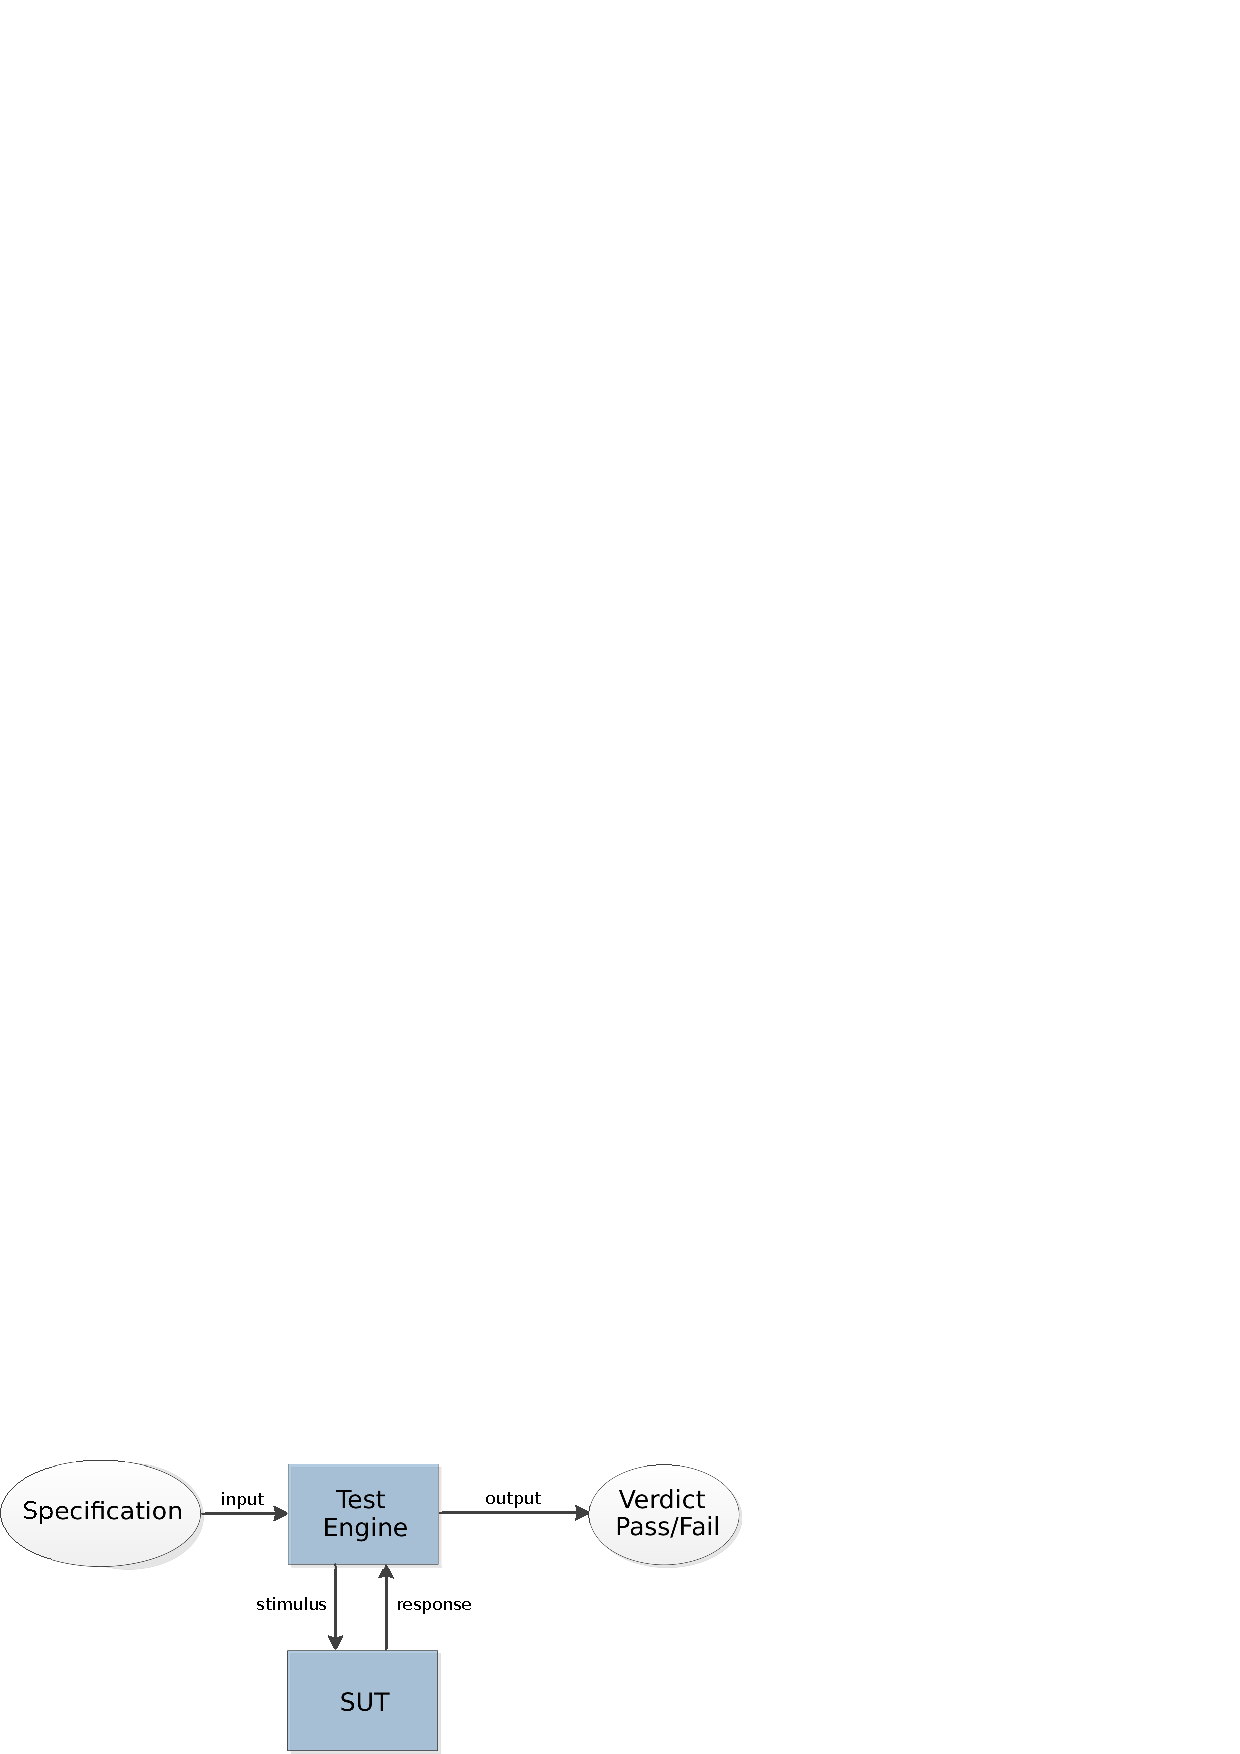
\includegraphics[width=0.75\textwidth]{mbt-on-the-fly.pdf}
  \end{center}
  \caption{A general 'on-the-fly' model-based testing setup}
  \label{fig:model_based_testing_on_the_fly}
\end{figure}\marginpar{A: Shrink font? V: Why?}

Variations of state machines and transition systems have been widely used as the underlying model for test generation. Other tools use the structure of data types to generate test data. 

The stucture of the rest of this section is as follows. First, previous work on model-based testing is given. Then, two types of models are introduced. These are basic formalisms useful to understand the models in the rest of the paper. Finally, the notion of \textit{coverage} is explained.

\subsection{Previous work}
Formal testing theory was introduced by De Nicola et al.~\cite{denicola:testing}. The input-output behavior of processes is investigated by series of tests. Two processes are considered equivalent if they pass exactly the same set of tests. This testing theory was first used in algorithms for automatic test generation by Brinksma~\cite{brinksma:testgeneration}. This led to the so-called \textit{canonical tester} theory. Tretmans gives a formal approach to protocol conformance testing (whether a protocol conforms to its specifications) in~\cite{Tretmans:conformancetesting} and an algorithm for deriving a sound and exhaustive test suite from a specification in~\cite{Tretmans:testgeneration}. A good overview of model-based testing theory and past research is given in "Model-Based Testing of Reactive Systems"~\cite{Broy:ModelBasedTesting}.

\subsection{Labelled Transition Systems}
A labelled transition system is a structure consisting of states with labelled transitions between them.
\vspace{5px}
\begin{definition}
A labelled transition system is a 4-tuple	$\langle Q, L, T, q_0\rangle$, where:
\begin{itemize}
\item $Q$ is a finite, non-empty set of states
\item $L$ is a finite set of labels
\item $T \in Q \times (L \cup \{\tau\}) \times Q$, with $\tau \notin L$, is the transition relation
\item $q_0 \in Q$ is the initial state.
\end{itemize}
We write $q \xrightarrow{\mu}q'$ if there is a transition labelled $\mu$ from state $q$ to state $q'$, i.e., $(q, \mu, q') \in T$. The informal idea of such a transition is that when the system is in state $q$ it may perform action $\mu$, and go to state $q'$. 
\end{definition}

\subsection{Input-Output Transition Systems}
A useful type of transition system for model-based testing is the Input-Output Transition System (IOTS) by Tretmans~\cite{Tretmans:testgeneration}. Assuming that implementations communicate with their environment via inputs and outputs, this formalism is useful for describing system behavior. IOTSs have the same definition as LTSs with one addition: each label $l \in L$ has a type $t \in T$, where $T = \{input, output\}$. Each label can therefore specify whether the action represented by the label is a possible input or an expected output of the system under test.

An example of such an IOTS is shown in Figure~\ref{fig:iots_example}. This system allows an input of 20 or 50 cents and then outputs tea or coffee accordingly. The inputs are preceded by a question mark, the outputs are preceded by an exclamation mark. This system is a specification of a coffee machine. A test case can also be described by an IOTS with special pass and fail states. A test case for the coffee machine is given in Figure~\ref{fig:iots_test}. The test case shows that when an input of '50c' is done, an output of 'coffee' is expected from the tested system, as this results in a 'pass' verdict. When the system responds with 'tea', the test case results in a 'fail' verdict. The pass and fail verdicts are two special states in the test case, which are sink states, i.e., once in either of those the test case cannot leave that state. 

Test cases should always reach a pass or fail state within finite time. This requirement ensures that the testing process halts.
\begin{figure}[ht]
  \begin{center}
    \subfloat[An IOTS]{\label{fig:iots_example}$\xymatrix{
    \bullet \ar[r]^{?50c} \ar[d]_{?20c} & \bullet \ar[d]^{\mathit{!coffee}} \\
    \bullet \ar[r]_{!tea}       & \bullet }$
}
    \subfloat[An IOTS test case]{\label{fig:iots_test}$\xymatrix{
    \bullet \ar[r]^{!50c} & \bullet \ar[r]^{\mathit{?coffee}} \ar[d]_{?tea} & {pass}\\
    & {fail}}$}
  \end{center}
  \caption{The specification of a coffee machine and a test case as an IOTS}
\end{figure}

\subsection{Coverage}\label{sec:coverage}
The number of tests that can be generated from a model is potentially infinite. Therefore, there must be a test selection strategy to maximize the quality of the tests while minimizing the time spent testing. Coverage statistics help with test selection. Such statistics indicate how much of the SUT is tested. When the SUT is a black-box, typical coverage metrics are state and transition coverage of the model~\cite{Lee:testing, Nachmanson:testing, Hasan:testing}.

As an example, let us calculate the coverage metrics of the IOTS test case example in~\ref{fig:iots_test}. The test case tests one path through the specification and passes through 3 out of 4 states and 2 out of 4 transitions. The state coverage is therefore 75\% and the transition coverage is 50\%.

Coverage statistics are calculated to indicate how adequately the testing has been performed~\cite{Zhu:coverage}. These statisics are therefore useful metrics for communicating how much of a system is tested.


	\section{Algebra}\label{sec:algebra}

Some basic concepts from algebra are described here. For a general introduction into logic we refer to~\cite{Huth:logic}.

A \textit{multi-sorted signature} $\langle S, F\rangle$ describes the function symbols and sorts of a formal language. $F$ is a set of function symbols, e.g. '+', '*', '=', '<', '0', '1'. Each $f\in F$ has an arity $n \in \mathbb{N}$, where a function symbol with arity $n = 0$ is called a constant symbol. The sort of a function symbol $f \in F$ is given by $\sigma(f) = S_1 ... S_n$. 

An \textit{algebra} $\mathcal{A} = \langle \mathbb{U}, \mathcal{F}\rangle$ has a non-empty set $\mathbb{U}$ of constants called a \textit{universe} and a set $\mathcal{F}$ of functions. A function $f_\mathcal{A}$ is typed $\mathbb{U}_1^{S_1} \times ... \mathbb{U}_{n-1}^{S_{n-1}} \rightarrow \mathbb{U}_n^{S_n}$, where $S$ is the sort of the function symbol given by the signature. For example, $<_\mathcal{A}: \mathbb{U}_\mathcal{A}^{int} \times \mathbb{U}_\mathcal{A}^{int} \rightarrow \mathbb{U}_\mathcal{A}^{bool}$ represents the 'less-than' comparison of two integers.
 
We define $\mathcal{V} = \mathcal{V}^{int} \sqcup \mathcal{V}^{real} \sqcup \mathcal{V}^{bool} \sqcup \mathcal{V}^{string}$ to be the set of \textit{variables}. \textit{Terms} over $V$, denoted $\mathcal{T}(V)$, are built from function symbols $F$ and variables $V \subseteq \mathcal{V}$. The definition of a term is:
\vspace{8px}\\
$\begin{array}{lrl}t & ::= & f(t_1 ... t_n) \\ & | & x\end{array}$, where $x$ is a constant.
\vspace{8px}\\
We write $var(t)$ to denote the set of variables appearing in a term $t \in \mathcal{T}(V)$. Terms $t\in \mathcal{T}(\emptyset)$ are called ground terms. An example of a term $\mathit{t}$ is $(x+y)$, with $var(t) = \{x,y\}$. The type of a term is given by:
\vspace{8px}\\
$\begin{array}{lll}\sigma: t \mapsto & s       & \mathit{if}\: t = x \in \mathcal{V}^S \\ 
                                     & s_{n+1} & \mathit{if}\: t = f(t_1 ... t_n) \mathit{\:and\:} \sigma(f) = S_1 ... S_{n+1}\mathit{,\:provided\:} \sigma(t_i) = S_i
\end{array}$
\vspace{8px}\\
A term with type $\mathbb{U}^{bool}$, is denoted as $\mathcal{R}(\mathcal{V})$. An example is $(x < y)$, where the result is $\mathit{true}$ or $\mathit{false}$.

A \textit{term-mapping} is a function $\sigma:\mathcal{V} \rightarrow \mathcal{T}(\mathcal{V})$. A \textit{valuation} $\nu$ is a function $\nu:\mathcal{V} \rightarrow \mathbb{U}$ that assigns constants to variables. For example, given an algebra, $\nu:\{(x \mapsto 1), (y \mapsto 2))\}$ assigns the constants 1 and 2 to the variables $x$ and $y$ respectively.
A valuation of a term given $\mathcal{A}$ is defined by $\nu(f(t_1 ... t_n)) \mapsto f_\mathcal{A}(\nu(t_1) ... \nu(t_n))$.

	\section{Symbolic Transition Systems}\label{sec:symbolic}
\textit{Symbolic Transition Systems} (STSs) combine a state oriented and data type oriented approach. These systems are used in practice in ATM and will therefore be part of GRATiS. First, previous work on STSs is given. The definition of STSs and IOSTSs follow. An example of an IOSTS is then given. Next, the transformation of an STS to an LTS is explained and illustrated by an example. This transformation is useful when comparing STSs to systems that are not STSs. Finally, different coverage metrics on STSs are explained.

\subsection{Previous work}
STSs are introduced by Frantzen et al.~\cite{Frantzen:Symbolic}. This paper includes a detailed definition, on which the definition in section~\ref{sec:sts_definition} is based. The authors also give a sound and complete test derivation algorithm from specifications expressed as STSs. Deriving tests from a symbolic specification or \textit{Symbolic test generation} is introduced by Rusu et al.~\cite{rusu:symbolic}. Here, the authors use \textit{Input-Output Symbolic Transition Systems} (IOSTSs). These systems are very similar to the STSs in~\cite{Frantzen:Symbolic}. However, the definition of IOSTSs we will use in this report is based on the STSs by~\cite{Frantzen:Symbolic}. A tool that generates tests based on symbolic specification is the STG tool, described in Clarke et al.~\cite{clarke:STG}.

\subsection{Definition}\label{sec:sts_definition}
An STS has \textit{locations} and \textit{switch relations}. If the STS represents a model of a software system, a location in the STS represents a state of the system, not including data values. A switch relation defines the transition from one location to another. The \textit{location variables} are a representation of the data values in the system. A switch relation has a \textit{gate}, which is a label representating the execution steps of the system. Gates have \textit{interaction variables}, which represent some input or output data value. Switch relations also have \textit{guards} and \textit{update mappings}. A guard is a term $t$, where any evaluation on $t$ with any valuation results in a value from $\mathbb{B} = \{true, false\}$. Such a term is denoted by $\mathcal{F}(\mathcal{V})$. The guard disallows using the switch relation when the evaluation of the term results in $false$. When the evaluation results in $true$, the switch relation of the guard is \textit{enabled}. An update mapping is a term-mapping of location variables. After the system switches to a new location, the variables in the update mapping will have the value corresponding to the evaluation of the term they map to.

\begin{definition}
A Symbolic Transition System is a tuple $\langle L,l_0,\mathcal{L},\imath,\mathcal{I},\Lambda,\rightarrow\rangle$, where:
\begin{itemize}
\item $L$ is a finite set of locations and $l_0 \in L$ is the initial location.
\item $\mathcal{L}$ is a finite set of location variables.
\item $\imath$ is a term-mapping $\mathcal{L} \rightarrow \mathcal{T}(\emptyset)$, representing the initialisation of the location variables.
\item $\mathcal{I}$ is a set of interaction variables, disjoint from $\mathcal{L}$.
\item $\Lambda$ is a finite set of gates. The unobservable gate is denoted $\tau (\tau \notin \Lambda)$; we write $\Lambda_\tau$ for $\Lambda \cup \{\tau\}$. The arity of a gate $\lambda\in\Lambda_\tau$, denoted $arity(\lambda)$, is a natural number. The parameters of a gate $\lambda\in\Lambda_\tau$, denoted $param(\lambda)$, are a tuple of length $arity(\lambda)$ of distinct interaction variables. We fix arity($\tau$) = 0, i.e. the unobservable gate has no interaction variables.
\item $\rightarrow \subseteq L \times \Lambda_\tau \times \mathcal{F}(\mathcal{V} \cup \mathcal{I}) \times \mathcal{L} \mapsto \mathcal{T}(\mathcal{L} \cup \mathcal{I}) \times L$, is the switch relation. We write $l\xrightarrow{\lambda,\phi,\rho}l'$ instead of $(l,\lambda,\phi,\rho,l')\in\rightarrow$, where $\phi$ is referred to as the guard and $\rho$ as the update mapping. We require $var(\phi) \cup var(\rho) \subseteq \mathcal{V} \cup param(\lambda)$, where $var$ is the collection of the variables used in the given guard or update mapping. We define $l\rightarrow \subset \rightarrow$ to be the outgoing switch relations from location $l$.
\end{itemize}
\end{definition}

An IOSTS can now easily be defined. The same difference between LTSs and IOTSs applies, namely each gate in an IOSTS has a type $t \in T$, where $T = \{input, output\}$. As with IOSTSs, each gate is preceded by a '?' or '!' to indicate whether it is an input or an output respectively.

\subsection{Example}\label{sec:sts_example}
In Figure~\ref{fig:example_sts} the IOSTS of a simple board game is shown, where two players consecutively throw a die and move along four squares. The 'init' switch relation is a graphical representation of the variable initialization $\imath$. The defining tuple of the IOSTS is:

$\langle\{throw, move\},throw,\{T, P, D\},\{T \mapsto 0, P \mapsto [0, 2], D \mapsto 0\},\{d, p, l\},\{?throw, !move\},\\
\{throw\xrightarrow{?throw, 1 <= d <= 6, D \mapsto d}move, move\xrightarrow{!move, T=p \land l=(P[p]+D)\%4, P[p] \mapsto l, T \mapsto p\%2}throw\}\rangle$

The variables $T, P$ and $D$ are the location variables symbolizing the player's turn, the positions of the players and the number of the die thrown respectively. The output gate $!move$ has $param = \langle p, l\rangle$ symbolizing which player moves to which location. The input gate $?throw$ has $param = \langle d\rangle$ symbolizing which number is thrown by the die. The switch relation with gate $?throw$ has the restriction that the number of the die thrown is between one and six and the update sets the location variable $D$ to the value of interaction variable $d$. The switch relations with gate $!move$ have the restriction that it must be the turn of the player moving and that the new location of the player is the number of steps ahead as thrown by the die. The update mapping sets the location of the player to the correct value and passes the turn to the next player. In Figure~\ref{fig:example_sts} the gates, guards and updates are separated by pipe symbols '|' respectively.

\begin{figure}[ht]
  \begin{center}
    $\xymatrix{
   \ar[rrrrr]^{init\,|\,true\,|\,T\,:=\,0;\,P\,:=\,[0,2];\,D\,:=\,0} &&&&& {throw} \ar@/^/[rrrrrrr]^{?throw(d:N)\,|\,1\,<=\,d\,<=\,6\,|\,D\,:=\,d} &&&&&&& {move} \ar@/^/[lllllll]^{!move(p:N,\,l:N) | T=p \land l = (P[p]\,+\,D)\,\%\,4\,|\,[p]\,:=\,l;\,T\,:=\,p\,\%\,2}}$

  \end{center}
  \caption{The STS of a board game example}
  \label{fig:example_sts}
\end{figure}

\subsection{STS to LTS transformation}\label{sec:sts_lts_trafo}
Consider an STS $S$ and its transformation LTS $L$. The following defines a mapping between $\mathcal{L}$, $\mathcal{V}$, $\mathcal{I}$ and $\rightarrow$ of $S$ to the states $Q$ and transitions $T$ of $L$.

\begin{definition}
  \item $\mu_l:(l \in L, \nu:\mathcal{V}) \mapsto q \in Q$
  \item $\mu_r:(r \in \rightarrow, \nu:\mathcal{I}) \mapsto t \in T$
\end{definition}

Finding the topology of $L$ is the next step of the transformation. For a switch relation $r$ from location $A$ to location $B$, a valuation of the location variables $\nu_l$ and interaction variables $\nu_i$, $\mu_l:(A,\nu_l)$ maps to a state $q$, where $q$ is the source state of a transition $t$, if the result of the evaluation $\epsilon:(\phi$ of $r, \nu_l \cup \nu_i)$ is true. $\nu_{l-new}$ is the new valuation of the location variables constructed by the evaluation of $\rho$ of $r$. Then, the target state $q'$ of $t$ is the state mapped by $\mu_l:(B,\nu_{l-new}$). The label of $t$ is a textual representation of $\lambda$ of $r$ and $\nu_i$. Applying this rule for the topology to all locations, switch relations and concrete values for the variables, results in $L$. The start state $q0$ of $L$ is the state mapped by $\mu_l:(l_0,\imath)$. All states not reachable from $q0$ are removed from $L$. When the number of possible valuations for $\mathcal{L}$ and $\mathcal{I}$ and the number of locations in an STS is considered to be finite, the transformation is always possible to an LTS with finite number of states.

An example of this transformation is shown in Figure~\ref{fig:example_trafo}. The label 'do(1)' in the LTS is a textual representation of the gate 'do' plus a valuation of the interaction variable 'd'. The transformation of a switch relation and concrete values to a transition is also called \textit{instantiating} the switch relation. Another term we will use for a switch relation with a set of concrete data values is an \textit{instantiated switch relation}.

\begin{figure}[ht]
  \begin{center}
    \subfloat[The STS]{\label{fig:trafo_sts}$\xymatrix{
   \ar[d]^{init\,|\,true\,|\,N\,:=\,0;} \\
   \bullet \ar@/^/[d]^{do(d:N)\,|\,1\,<=\,n\,<=\,2\,|\,N\,:=\,n} \\
   \bullet \ar@/^/[u]^{sub(i:N)\,|\,1\,<=\,i\,<=\,2\,|\,N\,:=\,N\,-\,i}}$
}\hspace{20px}
    \subfloat[The LTS]{\label{fig:trafo_lts}$\xymatrix{
   \fbox{N=0} \ar[rr]^{do(1)} \ar[dd]_{do(2)} && \fbox{N=1} \ar@(ul,ur)^{do(1)} \ar@(d,r)[ddll]^{do(2)} \\ \\
   \fbox{N=2} \ar@/^/[uurr]|-{do(1)} \ar@(dl,dr)[]_{do(2)}}$
}
  \end{center}
  \caption{An example of a transformation of an STS to an LTS}
  \label{fig:example_trafo}
\end{figure}

\subsection{Coverage}\label{sec:sts_coverage}
The simplest metric to describe the coverage of an STS is the location and switch-relation coverage, which express the percentage of locations and switch relations tested in the test run. Measuring state and transition coverage of an STS is possible using the LTS resulting from the STS transformation. However, this metric is not always useful, because the number of states and transitions in the LTS depend on the number of unique combinations of concrete values of the variables in the STS. This is potentially very large. For example, when the guards of the switch relations in Figure~\ref{fig:trafo_sts} are removed, the transformation leads to an LTS with a state and transition for each possible value of an integer. It is often unfeasable to test every data value in the STS. The most interesting data values to test can be found by \textit{boundary-value analysis} and \textit{equivalence partitioning}. For an explanation of these terms we refer to~\cite{Myers:2004}. Boundary-value analysis was found to be most effective by Reid~\cite{Reid:partitioning} in fault detection.

\textit{Data coverage} expresses the percentage of data tested in the test run, considering data to be similar if located in the same partition and a better representative of the partition if located close to the partition boundary. These properties of the tested data affect the data coverage percentage.

	\section{Graph Grammars}\label{sec:graph}
A \textit{Graph Grammar} (GG) is composed of a set of graph transformation rules. These rules indicate how a graph can be transformed to a new graph. These graphs are called \textit{host graphs}. The rules are composed of graphs themselves, which are called \textit{rule graphs}.

The rest of this section is ordered as follows: first, host graphs, rule graphs and graph transformation rules are explained. Then, the definition of a \textit{Graph Transition System} (GTS) is given. An example of a GG and a GTS is then given. Finally, the definition of IOGGs is given. For a more detailed overview of GGs, we refer to~\cite{Rensink:graph_grammars, Heckel2006187, Andries1999}.

In this report, we assume a universe of nodes $\Nodes = \GraphNodes \uplus \mathbb{U} \uplus \Variables \uplus 2^\Terms$\newnot{symbol:Nodes}, where $\GraphNodes$ is the universe of standard graph nodes. $\Edges$ is the universe of edges between two nodes in $\Nodes$.

\subsection{Host graphs}
A host graph $\hostGraph$ is a tuple $\langle \DefinedNodes, \DefinedEdges\rangle$\newnot{symbol:hostGraph}, where:
\begin{itemize}
  \item $\DefinedNodes \subseteq (\mathbb{W} \uplus \mathbb{U})$ is the node set of $\hostGraph$
  \item $\DefinedEdges \subseteq (\DefinedNodes\backslash\mathbb{U} \times \Labels \times \DefinedNodes)$ is the edge set of $\hostGraph$
\end{itemize}

\subsection{Rule graphs}
A rule graph $\ruleGraph$ is a tuple $\langle \DefinedRuleNodes, \DefinedRuleEdges \rangle$\newnot{symbol:ruleGraph}, where:
\begin{itemize}
  \item $\DefinedRuleNodes \subseteq (\Nodes \backslash \mathbb{U})$ is the node set of $\ruleGraph$
  \item $\DefinedRuleEdges \subseteq (\DefinedRuleNodes \times \Labels \times \DefinedRuleNodes$ is the edge set of $\ruleGraph$
\end{itemize}

In addition, the following must hold: $(\forall \node \in \DefinedRuleNodes \land \node \in 2^\Terms\: .\: var(\node) \subseteq \DefinedRuleNodes) \land (\forall \node \in \DefinedRuleNodes \land \node \in \Variables\: .\: \exists (\_, \_, \node) \in \DefinedRuleEdges$.

\subsection{Morphisms \& matches}
A graph $g$ has a \textit{morphism} to a graph $g'$ if there is a structure-preserving mapping from the nodes and the edges of $g$ to the nodes and the edges of $g'$ respectively. Such a mapping is called a \textit{morphism}. A node or edge $\node$ in graph $g$ is then said to have an \textit{image} in graph $g'$ and $\node$ is a \textit{pre-image} of the image. A \textit{match} is defined by a morphism from a rule graph to a host graph. A variable $\variable \in \Variables^{\sort}, \sort \in \Sorts$, has an image $i$ in a host graph if $i \in \mathbb{U}^{\sort}$. A node $\node \in 2^\Terms$ has an image $i$ in a host graph if $i$ is the valuation of all terms in $\node$. A graph $g$ has a partial morphism to a graph $g'$ if there are elements in $g$ without an image in $g'$.

\subsection{Graph transformation rules}\label{sec:graph_rules}
\vspace{5px}
\begin{definition}
A transformation rule $\ggrule \in \Rules$ is a tuple $\langle \mathit{LHS}, \mathit{NAC}, \mathit{RHS}, \ltsLabel \rangle$, where:
\begin{itemize}
  \item $\mathit{LHS}$ is a rule graph representing the left-hand side of the rule
  \item $\mathit{NAC}$ is a set of rule graphs representing the negative application conditions
  \item $\mathit{RHS}$ is a rule graph representing the right-hand side of the rule
  \item $\ltsLabel \in \Labels$ is the label of the rule
\end{itemize}
\end{definition}

A rule $R$ is applicable on a host graph $\hostGraph$ if its $\mathit{LHS}$ has a match in $\hostGraph$ and $\not\exists\,n \in \mathit{NAC}$ such that $n$ has a match in $\hostGraph$ and $\forall\,e \in \mathit{LHS}$, if $e$ has an image $i$ in $n$, and an image $j$ in $\hostGraph$, then $j$ should be an image of $i$.

This 'applicability' as defined here is refered to as a \textit{rule match}. After the rule match is applied to the graph, all elements in $\mathit{LHS}$ that do not have an image in $\mathit{RHS}$, are removed from $\hostGraph$ and all elements in $\mathit{RHS}$ that do not have a pre-image in $\mathit{LHS}$, are added to $\hostGraph$. This process, called a \textit{rule transition}, is denoted $\hostGraph \xrightarrow{\ggrule \in \Rules, \rulematch \in \RuleMatches}\hostGraph'$, where $\rulematch$\newnot{symbol:RuleMatches} is the rule match, i.e. the morphism of the $\mathit{LHS}$ to $\hostGraph$.

\subsection{Example}\label{sec:gts_example}
Figure \ref{fig:gg_example} shows an example of the initial graph $\startGraph$, one rule of a GG and the corresponding rule match. $\startGraph$ can be represented by $\langle\{n1,n2\},\{\langle n1,a,n1\rangle, \langle n1,A,n2\rangle,\langle n2,B,n2\rangle\}\rangle$. The $\mathit{LHS}$ of the rule has a match in $\startGraph$. Neither $\mathit{NAC1}$ and $\mathit{NAC2}$ have a match in $\startGraph$, because the edge with label $C$ does not exist in $\startGraph$. The new graph after applying the rule is $\hostGraph_1$.

\begin{figure}[ht]
  \begin{center}
    % To use this figure in your LaTeX document
% import the package groove/resources/groove2tikz.sty
%
% Special colors
\begin{tikzpicture}[
% Special color styles
scale=\tikzscale]
\node[node] (lhs)  at (2.200, 0.000) {\ml{\textbf{LHS} \\ $\xymatrix{
   r1 \ar@(dl,dr)[]_{A} \ar[r]^{a} & r2 \ar@(dl,dr)[]_{B}
}$
}};
\node[node] (n1)  at (-0.500, 0.000) {\ml{\textbf{NAC1} \\ $\xymatrix{
   \bullet \ar@(dl,dr)[]_{A} \ar[r]^{a} & \bullet \ar@(dl,dr)[]_{C}
}$
}};
\node[node] (n2)  at (-0.500, -1.500) {\ml{\textbf{NAC2} \\ $\xymatrix{
   \bullet \ar@(dl,dr)[]_{A} \ar[r]^{b} & \bullet \ar@(dl,dr)[]_{C}
}$
}};
\node[node] (g)  at (2.200, -2.000) {\ml{\textbf{$\startGraph$} \\ $\xymatrix{
   n1 \ar@(dl,dr)[]_{A} \ar[r]^{a} & n2 \ar@(dl,dr)[]_{B}
}$
}};
\node[node] (rhs)  at (5.000, 0.000) {\ml{\textbf{RHS} \\ $\xymatrix{
   \fbox{A} \ar[r]^{b} & \fbox{B}
}$
}};
\node[node] (g2)  at (5.000, -2.000) {\ml{\textbf{$\hostGraph_1$} \\ $\xymatrix{
   n1 \ar@(dl,dr)[]_{A} \ar[r]^{b} & n2 \ar@(dl,dr)[]_{B}
}$
}};
\path[edge] (lhs)  -- node[lab]{partial morphism} (n1) ;
\path[edge] (lhs)  -- node[lab]{partial morphism} (rhs) ;
\path[edge] (lhs)  -- node[lab]{partial morphism} (n2) ;
\path[edge] (g)  -- node[lab]{trafo} (g2) ;
\path[edge](lhs.south -| 2.200, -2.000) -- node[lab]{match} (g) ;
\path[edge](rhs.south -| 5.000, -2.000) -- node[lab]{match} (g2) ;
\userdefinedmacro
\end{tikzpicture}
\renewcommand{\userdefinedmacro}{\relax}

  \end{center}
  \caption{An example of a GG}
  \label{fig:gg_example}
\end{figure}

\subsection{Graph Transition Systems}
By repeatedly applying graph transformation rules to the start graph and all its consecutive graphs, a GG can be explored to reveal a \textit{Graph Transition System} (GTS). This transition system consists of graphs connected by rule transitions.
\vspace{5px}
\begin{definition}
A graph transition system is a tuple	$\langle \Graphs, \Rules, \RuleMatches, \RuleTransitions, \startGraph\rangle$, where:
\begin{itemize}
\item $\Graphs$\newnot{symbol:Graphs} is a set of graphs
\item $\Rules$\newnot{symbol:Rules} is a set of transformation rules
\item $\RuleMatches$ is a set of rule matches
\item $\RuleTransitions \in \Graphs \times \Rules \times \RuleMatches \times \Graphs$\newnot{symbol:RuleTransitions} is the rule transition relation
\item $\startGraph \in \Graphs$\newnot{symbol:startGraph} is the initial graph
\end{itemize}
\end{definition}

\subsection{Input-Output GGs}
In order to specify stimuli and responses with GGs, a definition is given for an \textit{Input-Output GG} (IOGG). Concretely, the IOGG places input and output labels on its rule transitions. Following the definition from IOLTSs, each rule transition label $l \in L$ has a type $\iotype \in \IOTypes$. Exploring an IOGG leads to an \textit{Input-Output Graph Transition System} (IOGTS).

	\section{Tooling}\label{sec:tooling}

\subsection{ATM}\label{sec:descriptionaxini}
ATM is a web-based model-based testing application, developed in the Ruby on Rails framework. It is used to test the software of several big companies in the Netherlands since 2006. It is under continuous development by Axini.

The architecture is shown graphically in Figure~\ref{fig:axini_tool}. It has a similar structure to the on-the-fly model-based testing tool architecture in Figure~\ref{fig:model_based_testing_on_the_fly}.

\begin{figure}[ht]
  \begin{center}
    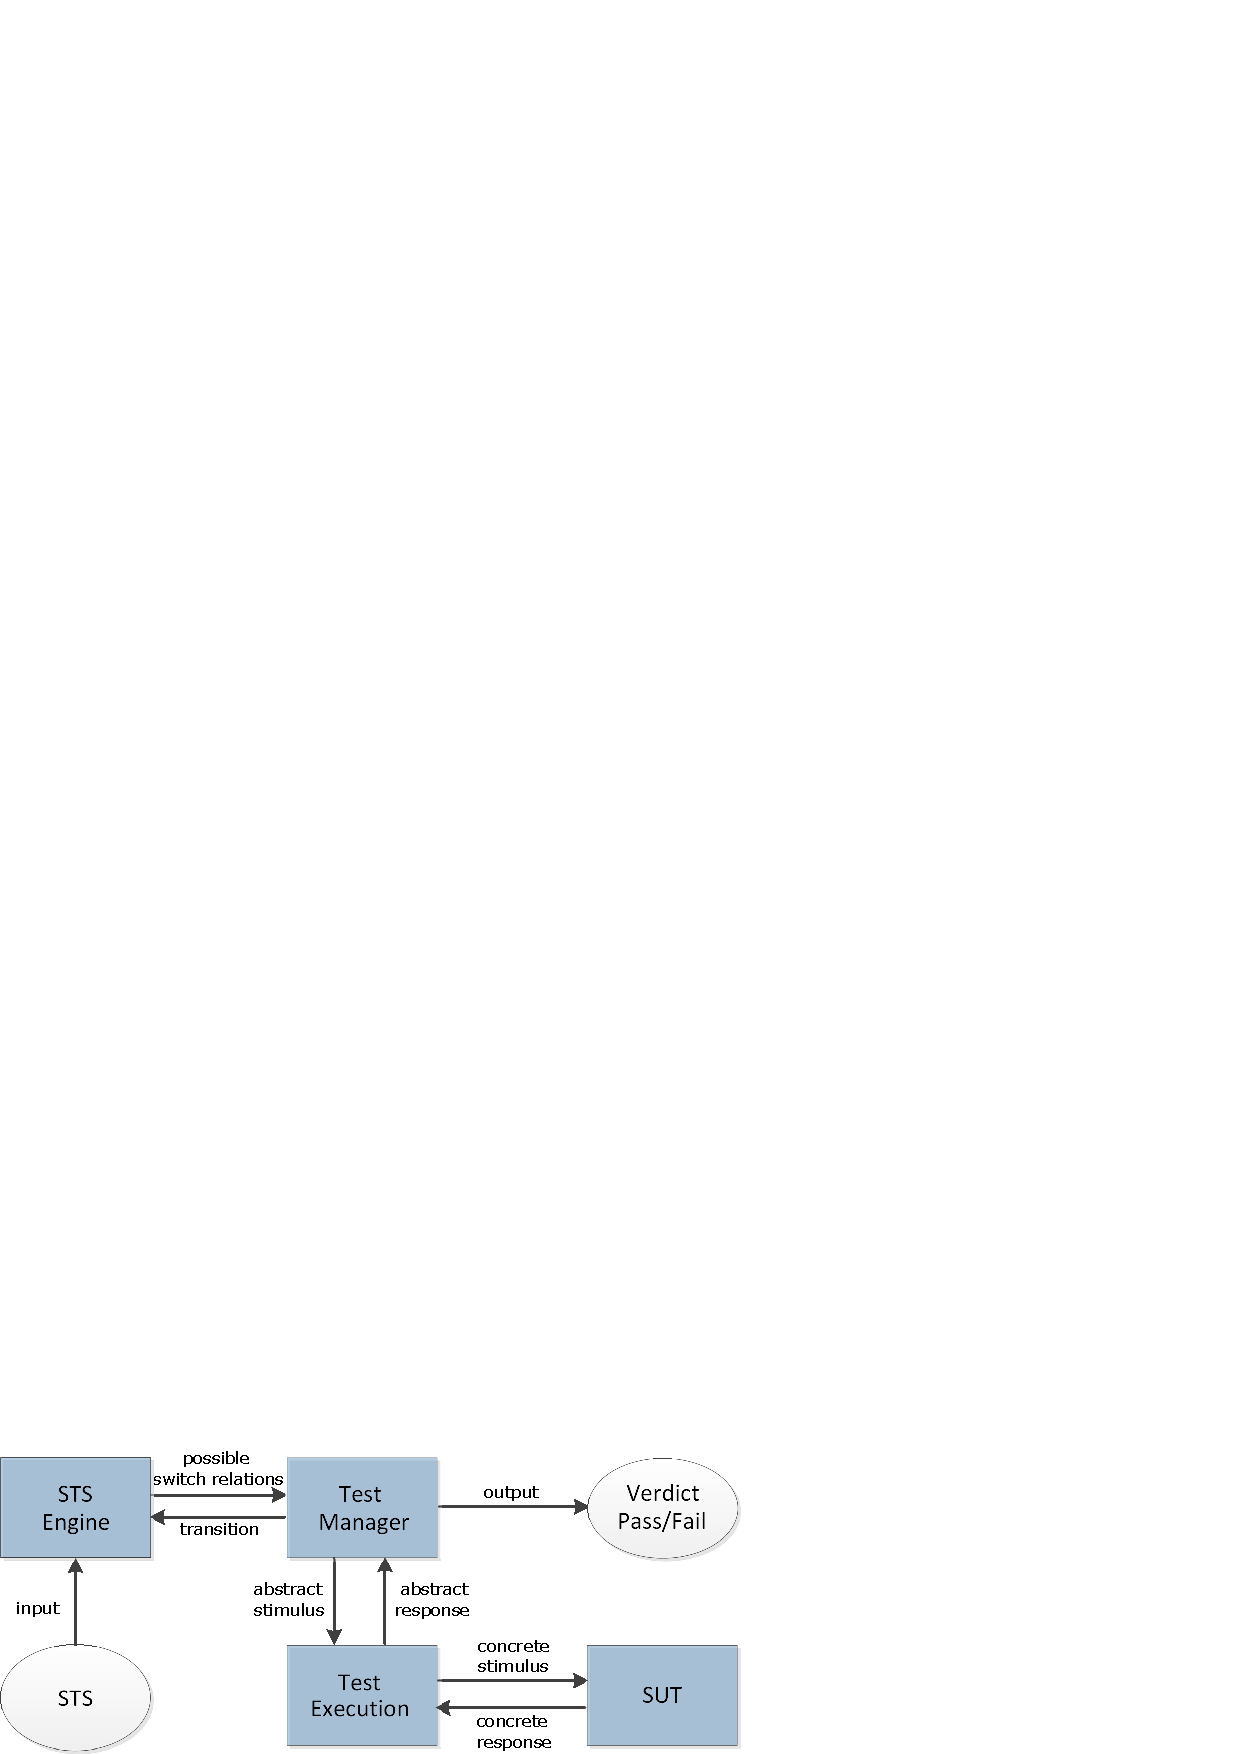
\includegraphics[width=0.75\textwidth]{axini_tool.pdf}
  \end{center}
  \caption{Architecture of ATM}
  \label{fig:axini_tool}
\end{figure}

The tool functions as follows: 
\begin{enumerate}
  \item An STS is given to an STS Engine, which keeps track of the current location and data values. It passes the possible switch relations from the current location to the Test Manager.
  \item The Test Manager chooses an enabled switch relation based on a test strategy, which can be a random strategy or a strategy designed to obtain a high location/switch relation coverage. The valuation of the variables in the guard are also chosen by a test strategy, which can be a random strategy or a strategy using boundary-value analysis. The choice is represented by an instantiated switch relation and passed back to the STS Engine, which updates its current location and data values. The communication between these two components is done by method calls.
  \item The gate of the instantiated switch relation is given to the Test Execution component as an \textit{abstract stimulus}. The term abstract indicates that the instantiated switch relation is an abstract representation of some computation steps taken in the SUT. For instance, a transition with label 'connect?' is an abstract stimulus of the actual setup of a TCP connection between two distributed components of the SUT. 
  \item The translation of an abstract stimulus to a concrete stimulus is done by the Test Execution component. This component provides the stimulus to the SUT. When the SUT responds, the Test Execution component translates this response to an abstract response. For instance, the Test Execution component receives an HTTP response that the TCP connect was succesful. This is a concrete response, which the Test Execution component translates to an abstract response, such as a transition with label 'ok!'. The Test Manager is notified with this abstract response.
  \item The Test Manager translates the abstract response to an instantiated switch relation and updates the STS Engine. If this is possible according to the model, the Test Manager gives a pass verdict for this test. Otherwise, the result is a fail verdict.
\end{enumerate}

\subsection{GROOVE}\label{sec:descriptiongroove}
GROOVE is an open source, graph-based modelling tool in development at the University of Twente since 2004~\cite{Rensink:GROOVE}. It has been applied to several case studies, such as model transformations and security and leader election protocols~\cite{Ghamarian:GROOVE}.

The architecture of the GROOVE tool is shown graphically in Figure~\ref{fig:groove_tool}. A graph grammar is given as input to the Rule Applier component, which determines the possible rule transitions. An Exploration Strategy can be started or the user can explore the states manually using the GUI. These components request the possible rule transitions and respond with the chosen rule transition (based on the exploration strategy or the user input). The Exploration Strategy can do an exhaustive search, resulting in a GTS. The graph states and rule transitions in this GTS can then be inspected using the GUI.

\begin{figure}[ht]
  \begin{center}
    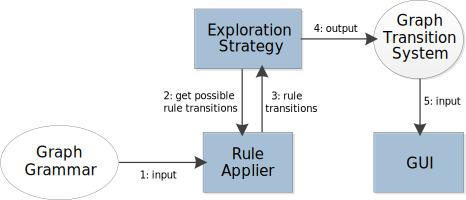
\includegraphics[width=0.75\textwidth]{groove_tool.pdf}
  \end{center}
  \caption{The GROOVE Tool}
  \label{fig:groove_tool}
\end{figure}


	
	\newpage
	\chapter{Design}\label{chapter:design}
	Section~\ref{sec:general-setup} shows the general setup of the GRATiS tool. Section~\ref{sec:offline-on-the-fly} describes two possible model generation techniques.


	\section{GRATiS Design}\label{sec:gratis-design}

\subsection{Tool architecture}
Show figure here of GRATiS architecture.

\subsection{Offline vs. on-the-fly model exploration}
The exploration of the graph grammar can be done in two ways: \textit{on the fly}, rule transitions are explored only when chosen by the Test Manager, or \textit{offline}, the graph grammar is transformed to an STS and sent to the Test Manager.

On-the-fly model exploration does not encounter the reachability problems discussed in the previous section. However, coverage statistics cannot be calculated on GRATiS, if the model exploration is done on the fly. The number of states/locations and transitions/switch relations the model has when completely explored are not known, so a percentage cannot be derived.

	
	\newpage
	\chapter{Graph Grammar to STS Algorithm}\label{chapter:gg_to_sts}
	\section{Requirements considerations}
From the research goals we derive three high level requirements:
\begin{enumerate}
\item The system should be able to perform model-based testing on GGs
\item The system should be validated so it should allow coverage metrics to be measured, because as seen in the previous chapter, coverage statistics are a useful and objective metric to describe how much of the model is tested
\item The system should be validated using case studies so it should be efficient enough to handle large models
\end{enumerate}

\paragraph*{IOGGs} In order to fulfill the first requirement, stimuli and responses have to be obtained from a GG. ATM uses an IOSTS, where the instantiated switch relations represent a stimulus to or a response from the SUT. GGs have no notion of inputs and outputs, therefore IOGGs have to be used as the model formalism. IOGGs can be explored to IOGTSs and the I/O labels of the IOGTS can be used to represent abstract stimuli/responses.

\paragraph*{On-the-fly vs. Offline exploration} The exploration of a GG can be done in two ways: \textit{on the fly}, rule transitions are explored only when chosen by ATM, or \textit{offline}, the GG is first completely explored and then sent to ATM. On-the-fly model exploration works well on large and even infinite models. However, coverage statistics cannot be calculated with this technique. The number of states (graphs) and rule transitions the model has when completely explored are not known, so a percentage cannot be derived. As coverage statistics are an important metric, the offline model exploration is chosen for GRATiS.

\paragraph*{Data values} An IOGTS can potentially be infinitely large, due to the range of data values. This is a potential risk for the validation of the system. A model that is more efficient with data values is an STS. The setup of GRATiS is therefore to transform the IOGG directly to an IOSTS. This transformation should be done efficiently to fulfill the third requirement. Note that the second requirement is still met, because location and switch relation coverage can be calculated on the IOSTS.

\paragraph*{} Taking these requirements into account, the method to achieve the goal of model-based testing on GGs is the following three steps:
\begin{enumerate}
\item Create an IOGG by assigning I/O types to the graph transformation rules of a GG
\item Create an IOSTS from the IOGG
\item Perform the model-based testing on the IOSTS
\end{enumerate}
The rest of this chapter describes a declaritive definition for creating an IOSTS from an IOGG.

\section{From IOGG to IOSTS}\label{sec:algorithm}
\subsection{Variables in GGs} 
The location variables in an STS represent an aspect of the modelled system. For instance, if a system keeps track of the number of items in containers, the STS modelling this system could have integer location variables $\mathit{items}_1..\mathit{items}_n$. GGs do not have this kind of variables. The variable nodes in rule graphs are used to match a value in a host graph, which is only available to that rule. A definition of persistent variables in GGs is needed in order to define location variables from an IOGG.

\vspace{10px}
\begin{definition} GG variables \\
A GG variable is a 3-tuple $\langle \variableAnchor, \variableEdge, \valueEdge\rangle$, where:
\begin{itemize}
\item \newnot{symbol:variableAnchor}$\variableAnchor \in \DefinedNodes\backslash\mathbb{U}$ is the \textit{variable anchor}.
\item \newnot{symbol:variableEdge}$\variableEdge \in \{\variableAnchor\} \times \Labels \times \{\variableAnchor\}$ is a self-edge of the variable anchor, called the \textit{variable edge}.
\item \newnot{symbol:valueEdge}$\valueEdge \in \{\variableAnchor\} \times \Labels \times \mathbb{U}\rangle$ is an edge from the variable anchor to a value node, called the \textit{value edge}.
\end{itemize}
\end{definition}
\vspace{10px}

The item/container example modelled in a graph grammar could be a graph node representing a container with an edge labelled `items' to an integer node. This is shown in Figure~\ref{fig:gg_vars_formal}. Using the labels of the variable anchor, variable edge and value edge, the variable $\langle \mathit{container, var1, items}\rangle$ is now represented by this graph. Figure~\ref{fig:gg_vars_groove} shows the same example in GROOVE. The variable edge is represented here by the flag \textit{var1}. Variable edges are represented by flags in GROOVE in the rest of this report. 

\begin{figure}[ht]
  \begin{center}
    \subfloat[Formal]{\label{fig:gg_vars_formal}\parbox[b]{4cm}{\centering$\xymatrix{
   \fbox{Container} \ar[rr]^{items} \ar@(ul,ur)^{var1} && \fbox{2}
}$
}}
    \subfloat[GROOVE]{\label{fig:gg_vars_groove}\parbox[b]{4cm}{\centering% To use this figure in your LaTeX document
% import the package groove/resources/groove2tikz.sty
%
% Special colors
\begin{tikzpicture}[
% Special color styles
scale=\tikzscale]
\node[node] (n0)  at (0.830, -0.620) {\ml{\textit{var1}\\Container\\items = 2}};
\userdefinedmacro
\end{tikzpicture}
\renewcommand{\userdefinedmacro}{\relax}
}}
  \end{center}
  \caption{Example of a GG variable}
  \label{fig:vars-in-ggs}
\end{figure}

\subsection{Graph exploration with point algebra} 
The IOGG cannot be directly made into an IOSTS, without using the IOGTS. To avoid the problem of a potentially infinitely large IOGTS, the point algebra is used. Using the point algebra when exploring a GG has two effects:
\begin{enumerate}
\item The host graphs that differ only in value nodes are collapsed into one
\item The variable nodes in rule graphs can have at most one image in the host graph
\end{enumerate}

\subsection{The IOGG to IOSTS definition} 
First the declaritive definition is given, then each part of the definition is described in more detail.
\vspace{10px}
\begin{definition} IOGG to IOSTS \\
Let $K$ be an IOGG. From $K$ we define an IOSTS $J$. The first step is to explore $K$ using the point algebra $\PointAlgebra$ to an IOGTS $O_\PointAlgebra$. The elements of $J$ can be obtained as follows:
\begin{itemize}
\item $\Locations = \Graphs$
\item $\initialLocation = \startGraph$
\item $\LocationVariables = \GGVariables$
\item $\Gates = \Rules$
\item $\InteractionVariables = \Variables$
\item $\Switches = \RuleTransitions$
\item guard
\item update mapping\marginpar{finish this list}
\end{itemize}
\end{definition}

\paragraph*{Locations} The locations abstract from data values, exactly like host graphs do under the point algebra. Therefore, the set of locations in $J$ are the set of host graphs in $O_\PointAlgebra$. The initial location in $J$ is also equal to the start graph of $O_\PointAlgebra$.

\paragraph*{Location variables} GG variables were defined to have location variables in GGs. Therefore, it is no surprise that the set of location variables in $J$ is exactly the set of GG variables in $O_\PointAlgebra$. This poses some constraints on creators/erasers for the variable anchors, variable edges and value edges. This is explained in detail in section~\ref{sec:constraints}.

\paragraph*{Gates}
The gate of a switch relation represents the stimulus to or response from the SUT. In an IOGG, the rules represent the stimuli and responses. Therefore, the set of gates $\Gates$ is chosen to be equal to the set of rules $\Rules$.

\paragraph*{Interaction variables}
Interaction variables are used by the gates to represent a stimulus or response variable. The variable nodes in rule graphs are this representation. The set of interaction variables $\InteractionVariables$ is chosen to be equal to the set of variable nodes $\Variables$. For a rule $\ggrule$ and all variable nodes $\Variables_\ggrule$ in $\mathit{LHS}$ of $\ggrule$, $arity(\ggrule) = |\Variables_\ggrule|$. \marginpar{need to define variable anchors in a graph, or variable labels in a graph}

\paragraph*{Switch relations}
A rule transition $\hostGraph \xrightarrow{\ggrule, \rulematch} \hostGraph' \in \RuleTransitions$ is mapped to a switch relation $(\hostGraph\xrightarrow{\ggrule, \guard, \updateMapping}\hostGraph') \in \Switches$. The guard and update mapping are constructed according to sections~\ref{sec:guards} and \ref{sec:updates} using $\ggrule$ and $\rulematch$. 

\paragraph*{Guard}\label{sec:guards}
The guard of a switch relation restricts the use of the switch relation based on the values of the variables. In a GG, a rule is restricted by the terms.\marginpar{need to define the term nodes in a graph} The variables used in the terms are interaction variables. Therefore, the first part of the guard is constructed by joining the terms for each term node by $\bigwedge_{\node \in \DefinedRuleNodes \cap \TermNodes}\bigwedge_{t_1, t_2 \in \node}t_1 = t_2$. Using a rule match $\rulematch$, the second part is constructed. For a $\mathit{LHS} = \langle \DefinedRuleNodes, \DefinedRuleEdges\rangle$ let $T$ be the smallest set of terms, such that $\langle \rulematch(\node), \ltsLabel \rangle = x \in T$ when:
\begin{itemize}
\item $x \in \Variables \cap \DefinedRuleNodes$
\item $\langle \node, \ltsLabel, x\rangle \in \DefinedRuleEdges$
\item $\rulematch(\node)$ is a variable anchor
\end{itemize}
Then, the terms are joined by $\bigwedge_{t\in T}t$.

\paragraph*{Update mapping}\label{sec:updates}
An edge with label $\ltsLabel$ from a variable anchor $\node$ to a value node can be erased from the graph and a new edge with label $\ltsLabel$ from $\node$ to a new value node can be created by a rule. This inidicates an update for the location variable given by $\langle \node, \ltsLabel \rangle$.\marginpar{make consistent with variable definition} In the rule graph, the $\mathit{RHS}$ of the rule has the pre-image of the $\node$ and the edge to a variable node, given by the interaction variable $x$. The update mapping for this example is: $\langle \node, \ltsLabel \rangle \mapsto x$.

\section{Rule priority}\marginpar{explain this clearer.}
This section covers a specific implementation issue of setting rule priorities in GROOVE.

The graphs are isomorphic under the point algebra, so they represent the same location. The STS of transforming this graph grammar is in Figure~\ref{fig:priority_sts_wrong}, with $\imath = \{x \mapsto 25\}$. This STS is wrong, because the 'sub' switch relation can be taken from the start.

\begin{figure}[ht]
  \begin{center}
    \input{./img/priority_sts_wrong.tex}
  \end{center}
  \caption{A wrong STS transformation of the graph grammar in Figure~\ref{fig:priority_gg}}
  \label{fig:priority_sts_wrong}
\end{figure}

The solution is shown in Figure~\ref{fig:priority_sts_right}. The negated guard of the 'add' switch relation is added to the 'sub' switch relation. The optimized guard for this switch relation is 'x >= 30' of course, but this shows the main principle: for each outgoing switch relation, the negated guard of all switch relations represented by higher priority rules must be added to the guard. So, the 'x < 30' guard is negated to '!(x < 30)' and added to yield the 'x > 10 \&\& !(x < 30)' guard. Note that if the 'add' switch relation had no guard, it would be applicable on all graph states with isomorphic abstractions. Therefore, the 'sub' switch relation would not exist, because the 'add' rule is always applicable whenever the 'sub' rule also is.

\begin{figure}[ht]
  \begin{center}
    $\xymatrix{
   \ovalbox{$l_0$} \ar@(ul,ur)[]^{?sub\,|\,x\,>\,10\:\&\&\:!(x\,<\,30)\,|\,x\,:=\,x\,-\,10} \ar@(dl,dr)[]_{?add\,|\,x\,<\,30\,|\,x\,:=\,x\,+\,10}
}$

  \end{center}
  \caption{A correct STS transformation of the graph grammar in Figure~\ref{fig:priority_gg}}
  \label{fig:priority_sts_right}
\end{figure}


	\section{Constraints}

This section describes the constraints on the algorithm of the previous section.

\subsection{Constraint 1: creator/eraser pairs}

\subsection{Constraint 2: no variables in NACs}

\subsection{Constraint 3: structural constraints on node creating rules}

	%\section{General setup}\label{sec:general-setup}
GROOVE has several exploration strategies for exploring a GG. The SymbolicStrategy is added as exploration strategy. It contains functionality to build an IOSTS from an IOGG. Figure~\ref{fig:tooling} shows the UML sequence diagram of GRATiS. The functionality of GROOVE and ATM as described in Figures~\ref{fig:axini_tool} and \ref{fig:groove_tool} is omitted where possible.

\begin{figure}[ht]
  \begin{center}
    \includegraphics[width=\textwidth]{gratis_diagram.pdf}
  \end{center}
  \caption{GRATiS sequence diagram}
  \label{fig:tooling}
\end{figure}

\begin{enumerate}
\item The user enters an IOGG in the RuleApplier.
\item The user sets the algebra family of the IOGG to to the point algebra. 
\item The user starts the SymbolicExplorationStrategy with a host and port. The communication between the RuleApplier and the strategy is omitted here. However, it should be noted that the point algebra is used by the RuleApplier here to create the rule transitions.
\item The SymbolicExplorationStrategy creates an IOSTS from the IOGTS and sends the IOSTS to the given host and port.
\item The IOSTS is given to the STSEngine. The ATMInterface takes the role of the UserInterface in ATM.
\item The ATMInterface starts the testing using a configurable depth parameter. The communication between the TestManager, STSEngine and Adapter is omitted here.
\item The TestManager returns the test results. The test results are stored in a database and are viewable through the user interface of ATM.
\end{enumerate}

\section{Description of added functionality}
This section covers in detail the added functionality to GROOVE and ATM. 

\subsection{GROOVE exploration strategy}
Figure~\ref{fig:esi-diagram} shows the class diagram of the added exploration strategy interface. The SymbolicExplorationStrategy has an exploration strategy such as the BreadthFirstStrategy to explore the GTS. The remote exploration strategy extends the symbolic exploration strategy.

The user starts the remote exploration strategy with a host and port. This strategy starts a breadth-first exploration strategy. This strategy explores the IOGG and notifies the remote strategy when there are no more rule transitions to explore. The symbolic strategy builds the IOSTS in Java objects using the explored rule transitions. The class diagram  of the IOSTS is given in section~\ref{sec:sts-setup}. The remote strategy sends the IOSTS in JSON format as a HTTP POST request to the interface at ATM.

The breadth-first exploration strategy and the symbolic strategy are loosely coupled, such that other strategies can also be used if desired.
 
\begin{figure}[ht]
  \begin{center}
    \includegraphics[width=0.35\textwidth]{strategy.pdf}
  \end{center}
  \caption{The class diagram of the exploration strategy interface}
  \label{fig:esi-diagram}
\end{figure}

\subsection{STSs}\label{sec:sts-setup}
Figure~\ref{fig:sts-diagram} shows the class diagram of the IOSTS in GRATiS. The IOSTS is composed of Location, SwitchRelation, Gate, Interaction- and LocationVariable classes. A Location object can be the start and target of any number of SwitchRelation objects. A SwitchRelation object has two Location objects; the start and target location. It also has one Gate object, which can belong to any number of SwitchRelation objects. A Gate object can have any number of InteractionVariable objects, but an InteractionVariable object belongs to only one Gate object. The IOSTS has a singleton class, the RuleInspector, which contains the functionality of building guards and updates from rule graphs.

\begin{figure}[ht]
  \begin{center}
    \includegraphics[width=0.5\textwidth]{STS.pdf}
  \end{center}
  \caption{The class diagram of the IOSTS in GRATiS}
  \label{fig:sts-diagram}
\end{figure}

Figure~\ref{fig:sts-objects} shows the object relations in accordance with the class diagram for the IOSTS in Figure~\ref{fig:example_sts}. Note that the links between the $\mathit{BoardGame}$ object and the Location, SwitchRelation, IOGate and InteractionVariable classes are not drawn for the sake of clarity.

\begin{figure}[ht]
  \begin{center}
    \includegraphics[width=0.8\textwidth]{STS_objects.pdf}
  \end{center}
  \caption{The object diagram of the IOSTS in Figure~\ref{fig:example_sts}}
  \label{fig:sts-objects}
\end{figure}

\subsection{ATM Interface}
The ATM interface is one component in the Ruby on Rails framework. The interface is a controller in this Model-View-Controller framework. Controllers handle the HTTP requests given by the framework. The interface receives the IOSTS POST request, builds the IOSTS as Ruby objects and initiates the test using this IOSTS as model.
	
	\newpage
	\chapter{Validation}\label{chapter:validation}
	This chapter covers the techniques used for the validation of the design. The validation is done through examples and a case-study, reported in section~\ref{sec:model-examples}. Possible measurements on models and the performance are reported in section~\ref{sec:measurements}.


	\section{Case Study}\label{sec:case-studies}

GRATiS has been applied to a real-life system Axini has worked on: a self-scan register. The self-scan register is a machine that automates the purchase of products at a supermarket. A customer can put his products on a conveyer belt and the system automatically calculates the price of the products. Then the customer pays and gets a receipt.\marginpar{add figure of machine}.

\subsection{Model}
A graph grammar is created for the self-scan register.add rules as examples. Add isues with modelling.Observation: GG is behavior-specification, was easy to adjust model according to specification. 

\subsection{Model comparison} 
Compare with STS. Nodes-Edges vs. Nodes-Edges? Halstaed's Software science? Compare transformed STS with original STS. Differences? But: transformed STS should be exactly the same! Depends on interpretation, bad-weather testing.


	%\section{Measurements}\label{sec:measurements}

\subsection{Model comparison}

\subsection{Benchmarks}

	\newpage
	\chapter{Conclusion}\label{chapter:conclusion}
	\begin{comment}
	\section{Summary}\label{sec:conclusion}
This report motivates the need of a research towards a model-based testing practice on Graph Transformation Systems. The goal will be to create a tool that allows automatic test generation on GTSs and assess the strengths and weaknesses of this test practice.

The first observations in this report demonstrate that GTSs can provide a nice visiualization of a system. However, the representation of data values and in a GTS were not   Increasing the complexity of the software system may change this. The transformation rules, given as separate graphs, provide a good overview of the behavior of the system. This feature should be beneficial in models for larger software systems.

The results also show an interesting automatic statespace reduction, namely the symmetry reduction. The second GTS of the example shows that also a purely arithmetic model can be built; this indicates the strength of the formalism.

The design phase is split into small steps that should break down the complexity of the entire implementation process. The validation with the use of the case studies emphasises the practicality of the tooling; the purpose of the test tools is to be used on real-world software systems. Finally, the experiments are a great indication of the usefulness of the tool towards software testers.
	This report shows the usability of Graph Grammars (GG) in model-based testing. The motivation to use GGs is supported by literature, as described in section~\ref{sec:gg_intro}, emphasizing the understandibility of graphs and the usefulness of graphs to express system states. Symbolic Transition Systems (STS), described in section~\ref{sec:symbolic}, are a useful formalism for computers. 

The overall goal of this research was to create a tool that can perform Model-Based Testing on GGs, using an existing graph transformation tool and a Model-Based Testing tool. The tools GROOVE and ATM, described in section~\ref{sec:tooling}, were used for this.

Model-based testing is a useful technique to test large software systems. The resulting tool, GRATiS, is an asset to the model-based testing paradigm. GROOVE is useful for modelling systems with Graph Grammars; ATM is used by several Dutch companies to test their software systems. The combination of the two tools allows Graph Grammars to be used as a model formalism for Model-Based Testing. The setup of GRATiS also allows other tools, such as JTorX, to replace ATM and work with the STSs produced by GRATiS.

\section{Research goals}
The research goals were:
\begin{enumerate}
  \item \textbf{Design}: Design and implement a system using ATM and GROOVE which performs Model-Based Testing on GGs.
  \item \textbf{Validation}: Validate the design and implementation using case studies and performance measurements.
\end{enumerate}

ATM and GROOVE were used to implement GRATiS. It generates an Input/Output STS (IOSTS) from the Input/Output GG (IOGG) in GROOVE and performs the testing on the IOSTS in ATM, described in chapter~\ref{chapter:implementation}. The tool was also validated using four example models and a larger case study, as described in chapter~\ref{chapter:validation}. Each case study featured an IOGG and a modelled IOSTS, each describing the same system behavior. The measurements done were: 
\begin{enumerate}
\item \textbf{Performance}: runtime and space requirements of the tool itself
\item \textbf{Simulation and redundancy}: comparing the generated IOSTS to the modelled IOSTS
\item \textbf{Model complexity}: comparing the IOGG to the modelled IOSTS
\item \textbf{Extendability}: extending the behavior of the system and comparing the new IOGG to the new IOSTS
\end{enumerate}
The performance measurement shows the technique implemented in GRATiS scales well; GRATiS can be used on large models without problem. The measurements on the generated IOSTS show that it is not always the smallest IOSTS possible, modelling an IOSTS by hand can often create smaller models. As these generated IOSTSs are hidden from the tester and only used by GRATiS to perform the Model-Based Testing, this is not a problem. The model complexity measurements, also on the extended models, were inconclusive. The measurement for model complexity, based on Halstead's software science, is a new concept for GGs and STSs. This measurement is further discussed below in `Contributions'.

The design requirements for GRATiS were: 
\begin{enumerate}
\item An IOGG must be used as the model; it must derive from the specification and be used for the testing.
\item It must be possible to measure the test progress/completion, by means of \textit{coverage} statistics (explained in detail in section~\ref{sec:coverage}).
\item The solution must be efficient: it should be usable in practice, therefore the technique should be scalable and the imposed constraints reasonable from a practical view point.
\end{enumerate}

The design requirements are all met, because:
\begin{itemize} 
\item the technique used in GRATiS proved effective for Model-Based Testing in the example cases and the case study
\item coverage can be measured on the generated IOSTS
\item the performance measurements show that the symbolic model can be generated from large IOGGs in a negligible time and that the technique scales well
\end{itemize}

\section{Contributions}
The contributions are:
\begin{enumerate}
\item A definition for variables in IOGGs in~\ref{def:gg_vars}
\item A technique to generate an IOSTS from an IOGG in section~\ref{sec:algorithm}
\item the tool GRATiS which implements the above-mentioned technique in chapter~\ref{chapter:implementation}
\item Model complexity measurements based on Halstead's Software Science for IOGGs and IOSTSs in section~\ref{sec:complexity_measurement}
\end{enumerate}

The next paragraphs describe each contribution listed above.

\paragraph*{GG variables}
Generating the variables in an IOSTS meant creating an extra definition for IOGGs, which allows persistent variables for GGs. These did not exist, because IOGGS can delete any node or edge, so also any variable definition in the graph. This gave problems to the technique, as described next.

\paragraph*{IOGG to IOSTS technique}
In order to generate an IOSTS from the IOGG such that it describes the same behavior, four constraints, described in section~\ref{sec:constraints}, had to be defined. IOGGs can dynamically add or delete these variables; something which was frequently desired to obtain the smallest and most intuitive models, but which complicates the generation of the IOSTS. Hence, constraints, on GG transformation rules were defined.

One of the example cases, a restaurant reservation system, suffered from the constraints the most. This example could not be modelled, because dynamically deleting and creating GG variables is not allowed by the constraints. The puzzle example on the other hand shows the strength of GGs the most: simple, intuitive rules opposed to a complicated transition system. This shows that some systems are more suitable to be modelled in IOGGs than others.

\paragraph*{GRATiS: the case study}
The case study done in this report on a self-scan register shows a real life example of a software system, successfully modelled as an IOGG. Here, the strength of behavioral rules is apparent: instead of state-transition thinking, the graph transformation rules allow each behavioral aspect of a software system to be modelled by one rule. For example, a `cash register not signed on' error can be given from any state the cash register is not signed on. In an IOGG, this is expressed by one rule, but generates many switch relations in the STS. Restrictions of where this rule does not apply can be easily added to the rule. In state-transition based models, many states and transitions are often needed to model the same behavior described by one GG rule. This shows that IOGGs are very useful when it comes to changing requirements: only few rules need to be adjusted to accomodate these changes.

\paragraph*{Model complexity}
Model complexity measurements were done on the IOGGs and IOSTSs of the example cases and case study. This did not reveal a clear difference in overall model complexity. However, it did show that IOGGs generally have more distinct operands, but less overall operators. The first part is due to the labels on nodes and edges, which describe the nature of the nodes and the relation between the nodes; these operands are not present in the IOSTSs. The second part can be explained by the repetition needed in IOSTSs to describe the same behavior as one IOGG rule.

	\section{Future work}\label{sec:future-work}
Better measurements to evaluate model complexity, such as sociological experiments, can be used to improve the usefulness of GGs in model-based testing. For instance, these measurements can be used to improve tools such as GROOVE, by making the GGs easier to create and understand.

When STSs are extended to allow more complex data structures, such as sets, maps and arrays, the definition of GG variables can also be extended. This should allow testers to viably model IOGGs for more software systems. Alternatively, other strengths of GGs can be explored, such as combining the consecutive application of the same rule into one, as was shown in the boardgame example.

More case studies on real-life software systems should be done, in order to establish and improve the usefulness of GRATiS to the model-based testing paradigm.
	\end{comment}
	\section*{ACKNOWLEDGEMENTS}

First I would like to thank my supervisors: Arend Rensink, Marielle Stoelinga, Axel Belinfante and Machiel van der Bijl.
All the energy and time put into giving me feedback, helping me when I got stuck and pushing me to do better has been greatly appreciated.

I would like to thank my current employers at Axini B.V. for providing the opportunity to do this master thesis and for giving me ample time to finish it.

I would like to also thank my fellow final year students: Freark van den Berg, Harold Bruintjes, Ronald Burgman, Paul Stapersma, Gerjan Stokkink and Lesley Wevers. Even though we were not always productive, the discussions while drinking coffee or beer have been fun.

Finally, I would like to thank my parents for providing me with a distraction-free environment and food, so I could concentrate completely on my full-time job and finishing my master thesis.


  \newpage
	\bibliography{bib/bibliography}{}
	\bibliographystyle{plain}
	\newpage
  \chapter*{List of Symbols\hfill} \addcontentsline{toc}{chapter}{List of Symbols}
\listofsymbols
\end{document}
